\documentclass[12pt]{article}
\usepackage[english]{babel}
\usepackage[utf8x]{inputenc}
\usepackage{amsmath}
\usepackage{graphicx}
\usepackage[colorinlistoftodos]{todonotes}
\usepackage{appendix}
\usepackage{graphicx}
\usepackage{xcolor}
\usepackage{float}
\usepackage{fancyhdr}
\usepackage{lastpage}
\usepackage{hyperref}
\usepackage{tabularx}

\widowpenalty 10000
\clubpenalty 10000

\bibliographystyle{alpha}

\definecolor{linkcol}{RGB}{42, 93, 176}
\hypersetup{
	colorlinks=true,
	linktoc=all,
	linkcolor=black,
	citecolor=teal,
	urlcolor=linkcol,
	bookmarksopen=true
}

\newcommand{\changeNumbering}[1]{
	\fancypagestyle{plain}{
		\renewcommand\headrulewidth{0pt}
		\fancyhf{}
		\fancyfoot[R]{\thepage\ of \pageref{#1}}
	}
	\fancyfoot[R]{\thepage\ of \pageref{#1}}
}
\pagestyle{fancy}
\fancyhf{}
\fancyhead[L]{SM1-SEM-U1-1-E17}
\fancyhead[R]{Group M}


\begin{document}

\listoftodos

\begin{titlepage}

\newcommand{\HRule}{\rule{\linewidth}{0.5mm}} % Defines a new command for the horizontal lines, change thickness here

\center % Center everything on the page
 

\textsc{\LARGE University of Southern Denmark}\\[1.5cm] % Name of your university/college
\textsc{\Large Software Engineering of Mobile Systems}\\[0.5cm] % Major heading such as course name
\textsc{\large Group m}\\[0.5cm] % Minor heading such as course title



\includegraphics[width=5cm]{images/ic_launcher}

%\HRule \\[0.4cm]
{ \huge \bfseries Give a Tip}\\[0.7cm] 
%\HRule \\[1.5cm]
 

\begin{minipage}[t]{0.4\textwidth}
\begin{flushleft} \large
\emph{Authors:}\\
Simon \textsc{H. Larsen}\\
Thomas \textsc{A. Lemqvist}\\
Veronika \textsc{Zemanova}\\
\end{flushleft}
\end{minipage}
~
\begin{minipage}[t]{0.4\textwidth}
\begin{flushright} \large
\emph{Supervisor:} \\
Mikkel \textsc{B. Kjærgaard}
\end{flushright}
\end{minipage}\\[2cm]
Student emails: \texttt{\{sila114, thlem14, vezem17\}@student.sdu.dk}\\[1.5em]
{\large December 21, 2017}\\[1.5cm] 


\includegraphics[width=.35\textwidth]{images/logo.png}\\[1cm]

\vfill 

\end{titlepage}
\changeNumbering{EndOfMainMatter}

\begin{abstract}
Your abstract
\end{abstract}

\vfill

\setcounter{tocdepth}{2}
\tableofcontents

\clearpage

% !TEX root = main.tex

\section{Introduction} \label{sec:intro}
% !TEX root = ../main.tex

This section introduces the motivation and context of the project, it describes the problem and the objective of the project, and shortly outlines the rest of the report.


\subsection{Motivation and Context}
This project has covered case number three, which works with the application 'Giv et Tip' \cite{GivEtTip}. The application is used by citizens of Odense Municipality, to report issues around the city, which the parks department is responsible for fixing. These issues include everything from potholes, to overfilled trash cans.
~\\

The objective for this case is to use mobile sensing and gamification to foster crowd sourcing of information, and keep people returning to the platform.
Mobile sensing is used in the existing application, to add extra data to the reports, such as a GPS location, to give the reports a precise geographic location, and to add images to the reports from the phone camera.

Gamification is needed in the current application, because there is no incentive to return to the platform, and users only use the application to report issues. By having a gamification system in place, the user will gain an incentive to return to the platform. This is done by adding game-like elements, such as progression, where users increase in rank and unlocks new features or content.


\subsection{Problem and Objective}
This project has worked with three problems with the current application, firstly validation of reports, which is how the municipality validates that the report is actually something they have to react upon, and fix. 
Secondly prioritization of reports, which is how the municipality prioritize the reported issues, and in which order they fix the reported issues. 
Lastly, the current application does not have an incentive to keep users on the platform, or gain new users, other than it being a easier way of reporting issues.
~\\

The objective for this project is to produce a prototype application, which will solve the report validation problem, by crowdsourcing the validations from the end users. The project will furthermore attempt to prioritize the reports, based on activity around reports. As well as as introducing some gamification elements to the platform, in order to incentivise new users, and to keep current users active on the platform. 

\subsection{Report Outline}
The report is structured as following: \autoref{sec:probdesc} describes the problems in greater detail. Section \ref{sec:solapp} will describe the solution to the problem on a high level. Section \ref{sec:analysis} will analyze the problem domain. Section \ref{sec:design} will build upon the analysis and describe the design decisions made. Section \ref{sec:impl} will describe the implementation of the solution. Section \ref{sec:verif} will verify weather the solution actually solves the problem. Section \ref{sec:reflect} will reflect upon the achieved results, and discuss them. Section \ref{sec:conclusion} will conclude the project and specify the directions for future works.

\section{Problem Description} \label{sec:probdesc}
% !TEX root = ../main.tex
This section will analyze and describe the problems, which was introduced in the introduction section, into greater detail. 
~\\

The validation of reports is a problem, as we assume that municipality workers have to spend time reading through reports, and validate them either based on submitted images, or travel to the location of the report to personally validate it. This process seems very time consuming and like a waste of municipality resources.

\begin{figure}[hbt]
\centering
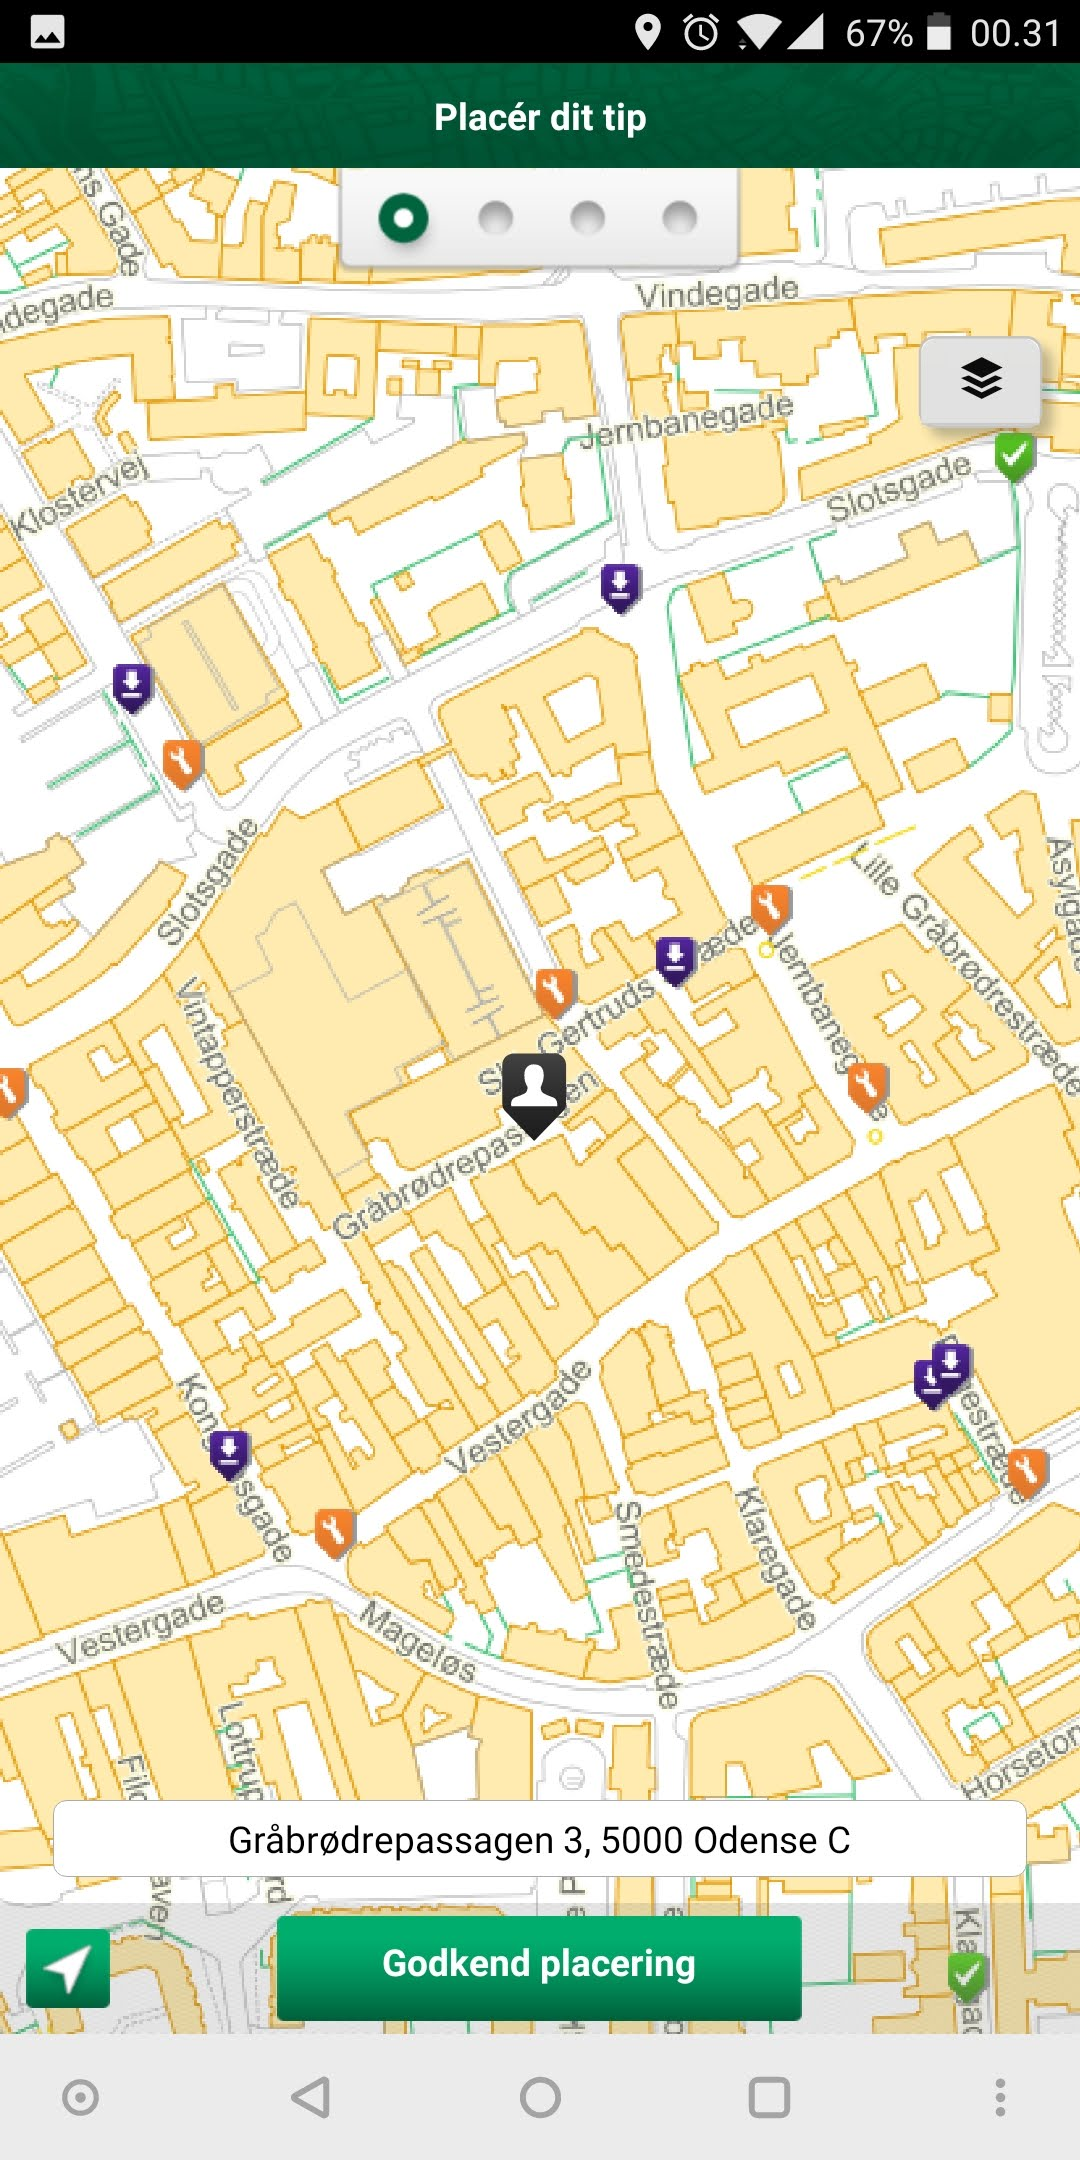
\includegraphics[width=5cm]{images/giv_et_tip_current_scr}
\caption{Image of the map screen in the current application.} \label{fig:current_app}
\end{figure}

In the current application, as \autoref{fig:current_app} shows, it is possible to see where other reports has been created, but there seems to be no way to get any information about these reports, other than the icons showing the report status.

The municipality also have a website which shows an overview of the current reports, but again, it does not offer any other functionality, for users to interact with the already reported issues. In order to contribute data to an already reported issue a user has to create a duplicate report with some more (accurate) information. This will eventually lead to more reports that the municipality workers have to validate.
~\\

The prioritization of reports is a problem, as we assume that the municipality workers have to dig through multiple reports and prioritize them. This process can cause a potentially dangerous issue, or an issue which affects more citizens, to become buried between the many other reports. 
~\\

The platform lacks an incentive for the users to use the platform, other than it being an easier way to report issues with. If there is no incentive to use the application, the amount of active users on the platform will decrease over time, which will result in a decrease in the amount of reports the municipality will receive.

\vspace{3em}

\hrule

This section has described the three problems that the project will try to solve. The solution for these problems will be elaborated upon in the next section.


\section{Solution Approach} \label{sec:solapp}
\todo[inline]{Describe the solution on a high-level (note: you can reuse and extend the pitch you already made).}.

%\section{Solution Description and Results} \label{sec:soldesc}
%% !TEX root = ../main.tex

This section will describe the solution on a lower level, and take it through the analysis, design, and implementation phases.

\subsection{Analysis}
% !TEX root = ../main.tex

\subsubsection{GUI Analysis}

\subsubsection{Actors}

\subsubsection{Use Cases}

\subsubsection{Requirements}

\subsubsection{Domain Model}


\subsection{Design}
% !TEX root = ../main.tex




\subsection{Implementation}
% !TEX root = ../main.tex




\section{Analysis} \label{sec:analysis}
% !TEX root = ../main.tex

\subsubsection{GUI Analysis}

\subsubsection{Actors}

\subsubsection{Use Cases}

\subsubsection{Requirements}

\subsubsection{Domain Model}


\section{Design} \label{sec:design}
% !TEX root = ../main.tex



\section{Implementation} \label{sec:impl}
% !TEX root = ../main.tex



\section{Verification} \label{sec:verif}
% !TEX root = ../main.tex



\subsection{Verification by Use}

\subsection{Energy Efficiency}

\section{Reflection and Discussion} \label{sec:reflect}
% !TEX root = ../main.tex
This section will reflect and discuss the reached solution, based upon tests and the results therefrom. It will elaborate on the parts of the problems, which was not solved. And finally reflect upon the project as a whole.

\subsection{Not Solved}
We wanted to create a web client, which should include a suite of administrative tools, for the municipality workers to use, to select issues to solve. In this web client, we would have solved the prioritization problem. But as we have not created this web client, as we deemed it out of the scope of the course, which focuses on mobile sensing.

Although it has not been implemented, we have made the architecture of our server application ready to serve a web client, and we believe that it would not be of great risk to implement such a client.
~\\

The lacking incentive for using the platform, has not been implemented in this prototype application, but it have been addressed, with the three solution suggestions from section X (ref 3). We have analyzed the three solutions and found both pros and cons for all implementations, and found that the lottery solution might promote cheating for personal materialistic gain, and would therefore not pursue that solution. And we found that the charity solution, was a good idea, as it could engage users, but it requires external investors in order to become a successful solution. Therefore, we find that the leaderboard solution is the easiest solution, as it do not require any external investors, and does not promote cheating by materialistic gain, but it might not be the most engaging gamification element. We therefore suggest that a combination of the three would be a great solution.
~\\

The reports in the current Giv et Tip application, has categories and images, both of which have not been implemented in this prototype, as it did not add any value to the problem domains. Although the categories could be used for weighing the prioritizations in the web client, so that more demanding categories would be weighed higher that less demanding categories.

\subsection{Project Reflection}
We have tried to utilize an agile approach to the development of the application, where we started by identifying the use cases, and assigned them to weekly sprints, and used a kanban system on GitHub, to keep track of the development progress. This system has worked out well for us, although we moved away from the weekly sprints, and just implemented the features, as we had time for it.
~\\

The project pitch at Odense Castle went well, this project won the “Giv et Tip” project category, and one of the judges, a developer from sweco, mentioned that we had a useful focus, with the crowdsourcing of verification.
~\\
The teamwork within the team, has worked out great, there has been great information and knowledge sharing throughout the process of this project.

\subsection{Known Issues}

\begin{description}
\item [Location permissions:] There is an issue with the location service, the first time the application is started, which renders the location service useless, as it never updates, unless the application is force-stopped, through the android application settings menu. This issue is caused by the lacking confirmation whether GPS is enabled on the first startup of the application. It could probably be fixed by waiting to start the location service until it is known that GPS is enabled.
\item [Shared preferences as storage:] The prototype makes excessive use of the shared preferences as data persistence. This is not optimal, and it would be much better to use SQLite, which is already included in android, for this purpose.
\item [Disabled location services:] There is another issue, which renders the location service useless. If the user disables the location services, in the android settings menu, the application will not prompt the user to re-enable it, when in the application is in focus, in order to make it usable again
\item [Download and storage of reports:] The background service is responsible for keeping report data up to date, by downloading report coordinates over time. It is currently configured to do this on a two hour interval. It would be nice to have some kind of manual update, which would offer users the option to force update the reports. Furthermore, these report coordinates is the only stored data about the reports. This means that every time the user needs to be shown report details, the application needs to download data for that report, and it is then thrown away afterwards.
\item [Settings:] The settings menu in the prototype only offers the option to tune the distance threshold to reports before a notification is shown. It could be great if there was some kinds of settings profiles in stead, which could offer e.g. a power saver mode, a  normal mode, and a power hungry mode. These profiles would be easier for an end user to understand the effects of.
\item [Geofences:] The prototype does not utilize the android api geo-fences, for figuring out which reports to calculate the distance to, but instead just calculates the distance to each and every report. This means that the application uses unnecessarily much processing power to calculate distances to reports, which are multiple kilometers away.
\item [Increased precision around already notified reports:] The prototype do not discriminate between new reports and reports it has already notified the user about, when it comes to calculating the distance to the reports. This means that it increases the GPS sensing precision, which is power consuming, for nothing, as the user will not be notified about the report anyways.
\end{description}

\subsection{Discussion}

The project aimed to solve the problem of validation of reports, prioritization of reports, and the lacking incentive of using the platform. All three problems have been addressed in this report, but only the validation problem solution has been implemented.

The validation problem was solved by implementing an infrastructure for crowdsourcing the validation. The infrastructure utilizes a background service, which runs continuously on the phone, and checks if there are nearby reports. The service then notifies the user when within 30 meters of a report. 
This service works as intended, members of the group have been receiving notifications, while not aware that the service ran in the background, about nearby reports. This proves that the service works as intended, as it should not bother the user other than when there are nearby reports.

As for the other two problems, this report has suggested different solutions, which have not been implemented, due to constraints in the scope and time available.

When developing for battery dependent devices like Android it is important to consider the energy efficiency of a solution for the device. A list of QAS and tactics is described in the tactics section \ref{sec:tactics}. In order to validate the tactics Battery Historian has been taken into use \cite{bathist}. This allows for measuring all of the activity on the Android device to be able to determine what is going on while using our app. 

While using battery historian a test was conducted. The device used for testing was a OnePlus 5T running Android 7.1.1. 

Thomas went out for a walk while having the app running in the background. Google Maps Timeline feature was used to track the path Thomas took while testing the application - it is worth mentioning that Google Maps nor any other location tracking service was running while Thomas was walking. \autoref{fig:thomas_walk} shows the path as well as a red circle, which marks the spot where reports were placed in our app.

\begin{figure}[H]
\centering
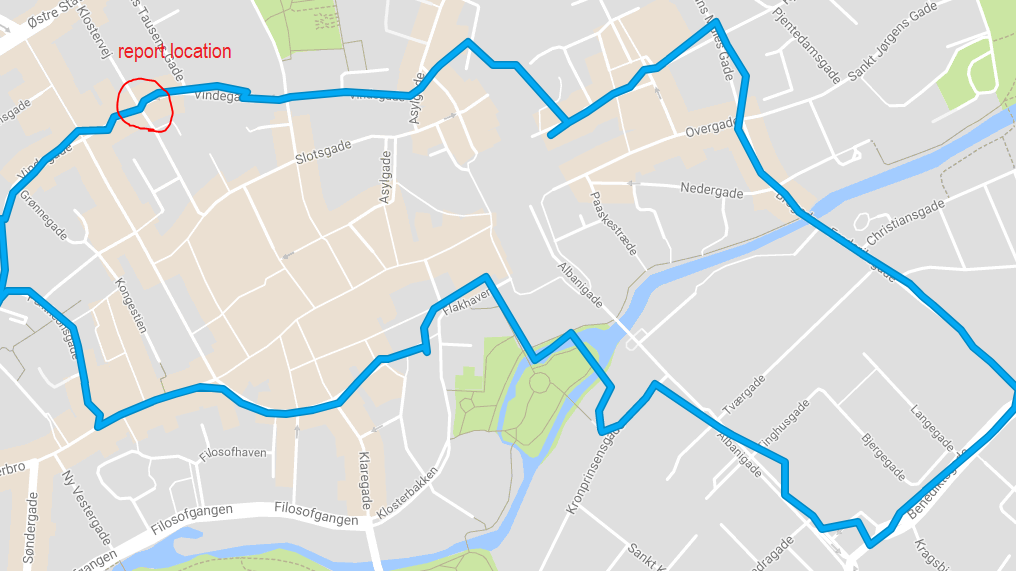
\includegraphics[width=.85\linewidth]{images/thomas_walk}
\caption{Map of the Thomas walk}
\label{fig:thomas_walk}
\end{figure}


Thomas got a notification as soon as he approached the red circle marked on figure \ref{fig:thomas_walk}. He approached the red circle somewhere around 1:27-1:29 PM according to Google Timeline. It is seen in figure \ref{fig:battery_stats_1} that the GPS is turned on at 1:27:08 PM until 1:30:50 PM. This fits very well into the timestamp provided by Google Timeline - this means that the GPS was turned on around the same time as Thomas was near the report.

\begin{figure}[H]
\centering
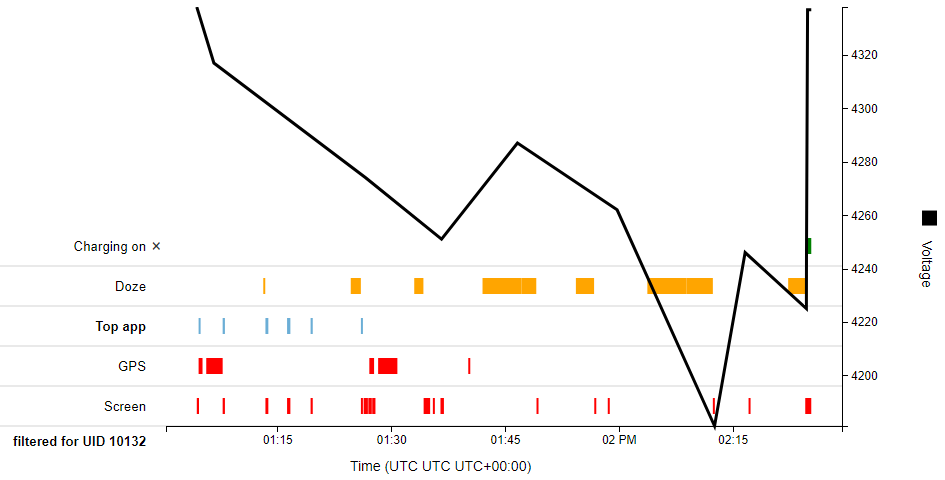
\includegraphics[width=\linewidth]{images/battery_hist}
\caption{Image from Battery Historian.} 
\label{fig:battery_stats_1}
\end{figure}

This confirms that the implementation of dynamic duty cycling works as the location sensor accuracy was changed when Thomas approached and moved away from the report. 

The accumulated discharge throughout the test was 7 percent with a test duration of 1 hour and 20 minutes. The power estimates throughout the test are shown in table \ref{fig:power_estimates}.


\begin{figure}[H]
\centering
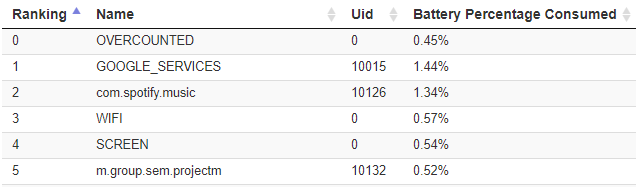
\includegraphics[width=\linewidth]{images/powerestimates}
\caption{Power estimates} 
\label{fig:power_estimates}
\end{figure}

Our solution comes in on a top 5 of the most battery consuming activities with 0.52\% battery consumption. This means that our app is responsible for 7.14\% of the battery consumption throughout the 1 hours and 20 minutes test. Compared to playing music using Spotify for the same duration, the battery consumption of our app is close to just one third of Spotify. 

Increasing the battery consumption by 7.14\% using our application would reduce the battery lifetime - of the device in question - by an estimated 1 hour and 20 minutes. Taking it from a 19 hour battery life to a 17 hour and 50 minutes lifetime. This seems like a fairly acceptable battery consumption considering that the application is relying on very precise GPS positioning. 

Potentially the battery consumption of the application could be reduced by optimizing the background service. Some of the ways to optimze the application are mentioned in the known issues section of the discussion. This includes using the geofencing to reduce activity recognition in the background. Other factors, methods, and tactics can also be investigated further to optimize battery usage.


\vspace{3em}
\hrule
Unsolved tasks has been stated as well as known issues. Project reflection described the agile approach to the project and the discussion section shows the validation and battery consumption test of the application. 

\section{Conclusion, Outlook and Future Work} \label{sec:conclusion}
% !TEX root = ../main.tex

\subsection{Conclusion}

\subsection{Outlook and Future Works}


%\nocite{*}
%\begin{multicols}{2}
\bibliography{ref}
%\end{multicols}
\addcontentsline{toc}{section}{References}
\label{sec:ref}
\label{EndOfMainMatter}
\newpage

% !TEX root = ../main.tex

\setcounter{page}{1}
\pagenumbering{Alph}
\changeNumbering{LastPage}
%\thispagestyle{empty}
\begin{appendices}

	\addtocontents{toc}{\protect\setcounter{tocdepth}{-1}}
	\section{Use Case Descriptions}
	% !TEX root = main.tex

% UC1
\begin{tabularx}{\textwidth}{|l|X|}
\hline
Name              & Register User \\ \hline 
Id                & UC1 \\ \hline
Description       & Allows unregistered users to create an account, and become a registered user.\\ \hline
Primary Actors    & Unregistered User \\ \hline
Secondary Actors  & Server \\ \hline
Preconditions     & The unregistered do not have an account \\ \hline
Main Flow         & {\footnotesize \begin{enumerate}
\item The unregistered user enters a username, and password.
\begin{enumerate}
\item Password has to be entered twice to make sure the user did not mistype it.
\end{enumerate}
\item The password is hashed for security reasons.
\item The username and hashed password is sent to the server.
\begin{enumerate}
\item Alternative flow: No connection to server.
\end{enumerate}
\item The server stores the password in the database.
\begin{enumerate}
\item Alternative flow: Username is already in use.
\end{enumerate}
\item end.
\end{enumerate}} \\ \hline
Postconditions    & The unregistered user has become a registered user. \\ \hline
Alternative Flows & 
No connection to Server:
{\footnotesize \begin{enumerate}
\item The user is informed of the missing connection.
\item end.
\end{enumerate}}
Username is already in use:
{\footnotesize \begin{enumerate}
\item The unregistered user is prompted to pick a new username.
\item Return to step 1 in main flow.
\end{enumerate}}
\\ \hline
\end{tabularx}

% UC2
\begin{tabularx}{\textwidth}{|l|X|}
\hline
Name              & Login \\ \hline 
Id                & UC2 \\ \hline
Description       & Allows user to login to the application. \\ \hline
Primary Actors    & Registered user \\ \hline
Secondary Actors  & Server \\ \hline
Preconditions     & The user is not logged into the application \\ \hline
Main Flow         &
{\footnotesize \begin{enumerate}
\item The user enters his username and password and selects the login option.
\item The password is hashed to match against the password hash in the database.
\item The username and hashed password is sent to the server.
\begin{enumerate}
\item Alternative flow: No connection to server.
\end{enumerate}
\item The server matches the username and hashed password with data from the database.
\begin{enumerate}
\item Alternative flow: Username or password does not match data in database.
\end{enumerate}
\item The user is logged in, and receives a user object from the server.
\item end.
\end{enumerate}} \\ \hline
Postconditions    & The registered user is now logged into the application. \\ \hline
Alternative Flows & 
No connection to Server:
{\footnotesize \begin{enumerate}
\item The user is informed of the missing connection.
\item end.
\end{enumerate}}
Username or password does not match data in database.
{\footnotesize \begin{enumerate}
\item The user is prompted to pick a new username.
\item Return to step 1 in main flow.
\end{enumerate}}
\\ \hline
\end{tabularx}

\begin{enumerate}
\item 
\end{enumerate}

% UC3
\begin{tabularx}{\textwidth}{|l|X|}
\hline
Name              & Create Report\\ \hline 
Id                & UC3 \\ \hline
Description       & Allows a registered user to report issues to the municipality \\ \hline
Primary Actors    & Registered user \\ \hline
Secondary Actors  & Server \\ \hline
Preconditions     & A registered user is logged in, and has encountered an issue, which the municipality is responsible for fixing. \\ \hline
Main Flow         &
{\footnotesize \begin{enumerate}
\item The user selects the ‘create report’ option.
\item The user enters a short description of the issue.
\item The user confirms the location of the report
\begin{enumerate}
\item Alternative flow: Wrong location.
\end{enumerate}
\item The user selects the submit report’ option.
\item The report is sent to the server.
\begin{enumerate}
\item Alternative Flow: No connection to the server.
\end{enumerate}
\item The user is informed of a successful submission.
\item end
\end{enumerate}} \\ \hline
Postconditions    & The report has been created. \\ \hline
Alternative Flows & 
Wrong Location:
{\footnotesize \begin{enumerate}
\item The user corrects the location by selecting the correct location.
\item Return to step 4 in main flow.
\end{enumerate}}
No connection to Server:
{\footnotesize \begin{enumerate}
\item The user is informed of the missing connection.
\item end.
\end{enumerate}}
\\ \hline
\end{tabularx}

% UC4
\begin{tabularx}{\textwidth}{|l|X|}
\hline
Name              & Change Settings \\ \hline 
Id                & UC4 \\ \hline
Description       & Allows users to change the distance threshold for receiving notifications. \\ \hline
Primary Actors    & User \\ \hline
Secondary Actors  & NA \\ \hline
Preconditions     & User wishes to change the distance needed to reports, in order to receive notifications \\ \hline
Main Flow         &
{\footnotesize \begin{enumerate}
\item The user selects the ‘settings’ option.
\item The user selects the distance threshold.
\item end.
\end{enumerate}} \\ \hline
Postconditions    & The distance threshold needed is updated. \\ \hline
Alternative Flows & NA \\ \hline
\end{tabularx}

% UC5
\begin{tabularx}{\textwidth}{|l|X|}
\hline
Name              & View Report \\ \hline 
Id                & UC5 \\ \hline
Description       & Allows users to view report details, such as description, comments and votes. \\ \hline
Primary Actors    & User \\ \hline
Secondary Actors  & Server \\ \hline
Preconditions     & The user wishes to see information about a report. \\ \hline
Main Flow         &
{\footnotesize \begin{enumerate}
\item The user selects a report on the map to see.
\item The application collects the newest data on the report from the server.
\begin{enumerate}
\item Alternative flow: No connection to server.
\end{enumerate}
\item The report is is shown to the user.
\item end.
\end{enumerate}} \\ \hline
Postconditions    & The user can see the report details. \\ \hline
Alternative Flows & 
No connection to Server:
{\footnotesize \begin{enumerate}
\item The user is informed of the missing connection.
\item end.
\end{enumerate}}
\\ \hline
\end{tabularx}

% UC6
\begin{tabularx}{\textwidth}{|l|X|}
\hline
Name              & View Leaderboard \\ \hline 
Id                & UC6 \\ \hline
Description       & Allows users to see the leaderboard standings. \\ \hline
Primary Actors    & User \\ \hline
Secondary Actors  & Server \\ \hline
Preconditions     & The user wants to see the leaderboard \\ \hline
Main Flow         &
{\footnotesize \begin{enumerate}
\item The user selects the ‘view leaderboard’ option.
\item The application collects the newest information from the leaderboard.
\begin{enumerate}
\item Alternative flow: No connection to server.
\end{enumerate}
\item The leaderboard is shown to the user.
\item end.
\end{enumerate}} \\ \hline
Postconditions    & The user can see the leaderboard. \\ \hline
Alternative Flows & 
No connection to Server:
{\footnotesize \begin{enumerate}
\item The user is informed of the missing connection.
\item end.
\end{enumerate}}
\\ \hline
\end{tabularx}

% UC7
\begin{tabularx}{\textwidth}{|l|X|}
\hline
Name              & Validate Report \\ \hline 
Id                & UC7 \\ \hline
Description       & Allows users to validate reports, by giving them an upvote or downvote. \\ \hline
Primary Actors    & Registered user \\ \hline
Secondary Actors  & Server \\ \hline
Preconditions     & The user is viewing a report, or have received a notification from based on his proximity to a report. \\ \hline
Main Flow         &
Precondition = View report:
{\footnotesize \begin{enumerate}
\item The user selects either the 'upvote' or the 'downvote' option on the report.
\item The vote is sent to the server.
 \begin{enumerate}
\item Alternative Flow: No connection to server.
\end{enumerate}
\item end.
\end{enumerate}}
Precondition = notification:
{\footnotesize \begin{enumerate}
\item The user selects the ‘confirm’ or the ‘deny’ option in the notification.
\item The vote is sent to the server.
 \begin{enumerate}
\item Alternative Flow: No connection to server.
\end{enumerate}
\item end.
\end{enumerate}} 
\\ \hline
Postconditions    & The user has validated the report \\ \hline
Alternative Flows & 
No connection to Server:
{\footnotesize \begin{enumerate}
\item The user is informed of the missing connection.
\item Validation option is stored, for later retry
\item end.
\end{enumerate}}
\\ \hline
\end{tabularx}

% UC8
\begin{tabularx}{\textwidth}{|l|X|}
\hline
Name              & Comment on Report \\ \hline 
Id                & UC8 \\ \hline
Description       & Allows users to comment on each others reports, to add more information to the reports \\ \hline
Primary Actors    & Registered user \\ \hline
Secondary Actors  & Server \\ \hline
Preconditions     & The user is viewing a report, or have received a notification from based on his proximity to a report. \\ \hline
Main Flow         &
Precondition = View report:
{\footnotesize \begin{enumerate}
\item The user enters a comment for the report.
\item The user selects the 'submit comment' option
\item The comment is sent to the server
 \begin{enumerate}
\item Alternative Flow: No connection to server.
\end{enumerate}
\item end.
\end{enumerate}}
Precondition = notification:
{\footnotesize \begin{enumerate}
\item User selects the 'comment' option in the notification.
\item The user enters a comment for the report.
\item The user selects the 'submit comment' option
\item The comment is sent to the server
 \begin{enumerate}
\item Alternative Flow: No connection to server.
\end{enumerate}
\item end.
\end{enumerate}} 
\\ \hline
Postconditions    & The user has submitted a comment to the report. \\ \hline
Alternative Flows & 
No connection to Server:
{\footnotesize \begin{enumerate}
\item The user is informed of the missing connection.
\item Comment is stored, for later retry
\item end.
\end{enumerate}}
\\ \hline
\end{tabularx}

% UC9
\begin{tabularx}{\textwidth}{|l|X|}
\hline
Name              & Display Report Notification \\ \hline 
Id                & UC9 \\ \hline
Description       & Allows the application to send notifications to the user, if he is within his set distance threshold of a report. \\ \hline
Primary Actors    & Location \\ \hline
Secondary Actors  & NA \\ \hline
Preconditions     & The user has location services enabled. \\ \hline
Main Flow         &
{\footnotesize \begin{enumerate}
\item The distance from the user’s current location is within the set threshold
\item The application checks if the user has already contributed to this report.
\begin{enumerate}
\item Alternative flow: Alternative Flow: User already contributed to report:
\end{enumerate}
\item The application checks if the user has been shown this report before
\begin{enumerate}
\item Alternative Flow: Report already shown.
\end{enumerate}
\item The application gets the latest information about the report.
\begin{enumerate}
\item Alternative Flow: No connection to server.
\end{enumerate}
\item The user is asked to validate the report.
\item end.
\end{enumerate}} \\ \hline
Postconditions    & A notification is shown to the user, and he can respond to ut with UC7 or UC8. \\ \hline
Alternative Flows & 
User already contributed to report:
{\footnotesize \begin{enumerate}
\item end.
\end{enumerate}}
Report already shown:
{\footnotesize \begin{enumerate}
\item end.
\end{enumerate}}
No connection to Server:
{\footnotesize \begin{enumerate}
\item end.
\end{enumerate}}
\\ \hline
\end{tabularx}
	

\end{appendices}



\end{document}